


% !TeX spellcheck = pt_BR
\documentclass{llncs}
\usepackage{llncsdoc}


\usepackage{graphicx}
\usepackage{indentfirst}
\usepackage{subfig}
\usepackage{listings}
\usepackage{url}
\usepackage{color}


\definecolor{dkgreen}{rgb}{0,0.6,0}
\definecolor{gray}{rgb}{0.5,0.5,0.5}
\definecolor{mauve}{rgb}{0.58,0,0.82}

\lstset{frame=tb,
  language=Prolog,
  aboveskip=3mm,
  belowskip=3mm,
  showstringspaces=false,
  columns=flexible,
  basicstyle={\small\ttfamily},
  numbers=none,
  numberstyle=\tiny\color{gray},
  keywordstyle=\color{blue},
  commentstyle=\color{dkgreen},
  stringstyle=\color{mauve},
  breaklines=true,
  breakatwhitespace=true
  tabsize=3
}




\begin{document}


\title{Hoo-Doo Solver}

\author{Daniel Mendon\c{c}a e Jos\'{e} Pedro Moreira}

\institute{FEUP-PLOG, Turma 3MIEIC9, Grupo 123}

\maketitle
%
\begin{abstract}
Este projecto consiste na implementa\c{c}\~{a}o de um \textit{solver} para o jogo de tabuleiro \textit{Hoo-Doo}, jogo esse que consiste em colocar numa matriz de lado n, v\'{a}rios exemplares de n tipos de pe\c{c}as por forma a que n\~{a}o existam duas pe\c{c}as iguais na mesma linha,coluna ou diagonal. O solver que nos propomos a desenvolver funciona para uma dimens\~{a}o arbitr\'{a}ria do tabuleiro. A implementa\c{c}\~{a}o foi feita usando Prolog, mas concretamente a plataforma \emph{Sicstus Prolog}  tendo sido usados para tal os m\'{o}dulos desta mesma ferramenta para Programa\c{c}\~{a}o em L\'{o}gica com Restri\c{c}\~{o}es sobre dom\'{i}nios finitos. Com a execu\c{c}\~{a}o do mesmo, e olhando aos seus resultados verific\'{a}mos os benef\'{i}cios de usar PLR para resolu\c{c}\~{a}o de problemas semelhantes a este.
\end{abstract}
%
\section{Introdu\c{c}\~{a}o}
\paragraph*{}
O Hoo-Doo \'{e} um jogo de tabuleiro criado nos anos 50 e que deriva do popular N Queens. Dependendo da sua dimens\~{a}o, pode ter v\'{a}rias, uma ou at\'{e} nenhuma resolu\c{c}\~{a}o se n\~{a}o forem usadas \emph{pegs} transparentes. Quando foi lan\c{c}ado o jogo de tabuleiro Hoo-doo, os seus criadores ofereciam 1000\$ \`{a} primeira pessoa que conseguisse resolver um tabuleiro de 8x8 sem recurso a \emph{pegs} transparentes, e, os elementos deste grupo acharam que seria interessante e at\'{e} certo ponto divertido verificar como a implementa\c{c}\~{a}o deste jogo em Prolog, usando restri\c{c}\~{o}es seria uma mais valia para vencer o pr\'{e}mio que era na altura oferecido. Apesar das poucas regras do jogo, a resolu\c{c}\~{a}o dos puzzles pode ser penosa. Num tabuleiro de oito posi\c{c}\~{o}es encontram-se 1.817.1052 combina\c{c}\~{o}es poss\'{i}veis, e nem sempre, noutros tamanhos h\'{a} solu\c{c}\~{a}o poss\'{i}vel.
\paragraph*{}
Apesar de ter sido realizada uma pesquisa sobre outras implementa\c{c}\~{o}es deste jogo de tabuleiro, nenhuma foi encontrada. A informa\c{c}\~{a}o sobre o jogo e solu\c{c}\~{o}es tamb\'{e}m \'{e} praticamente inexistente, pelo que n\~{a}o nos foi poss\'{i}vel comparar a nossa abordagem com outras realizadas. Na nossa implementa\c{c}\~{a}o, o problema \'{e} resolvido com a aplica\c{c}\~{a}o de restri\c{c}\~{o}es a linhas, colunas e ambas as diagonais poss\'{i}veis para cada posi\c{c}\~{a}o do tabuleiro .
\paragraph*{}
Para testar o programa criado, deve ser chamado o predicado start. Na implementa\c{c}\~{a}o realizada do jogo, tamb\'{e}m temos a possibilidade de procurar solu\c{c}\~{o}es para tabuleiros rect\^{a}ngulares, situa\c{c}\~{a}o n\~{a}o prevista no jogo original.
 
O trabalho desenvolvido pelos elementos do grupo tem tr\^{e}s partes distintas:
\begin{itemize}
\item Parte de visualiza\c{c}\~{a}o do jogo, em muito semelhante ao j\'{a} desenvolvido num outro trabalho para a disciplina;
\item Parte do \emph{solver}, que resolve o tabuleiro que lhe \'{e} passado;
\item Parte de convers\~{a}o de tabuleiro \emph{flat} para tabuleiro bi-dimensional e vice-versa.
\end{itemize}

Na implementa\c{c}\~{a}o do jogo \'{e} suportado o funcionamento em dois modos, um que n\~{a}o usa \emph{pegs} transparentes, e outro que usa, tentando no entanto minimizar a sua utiliza\c{c}\~{a}o.

%

\section{Descri\c{c}\~{a}o}
%
\paragraph*{}
O jogo Hoo-Doo foi criado pela empresa Tryne Sales Inc., New York City, lan\c{c}ado na d\'{e}cada de 50. Hoo-Doo \'{e} um jogo de tabuleiro, para um \'{u}nico jogador, normalmente quadrado e que tem pelo menos tantas cores quanto o n\'{u}mero de colunas no tabuleiro, e o numero de \emph{\emph{pegs}} de cada cor  \'{e} tamb\'{e}m o n\'{u}mero de colunas do tabuleiro. Os tamanhos de tabuleiro mais frequentes s\~{a}o os de 4x4, 6x6 e 8x8.
\paragraph*{}O jogo tem como in\'{i}cio um tabuleiro vazio, e o objectivo \'{e} preencher todas as posi\c{c}\~{o}es do tabuleiro com as \emph{pegs} dispon\'{i}veis, sem nunca repetir pe\c{c}as da mesma cor na mesma linha, coluna, ou qualquer uma das diagonais. Para auxiliar na resolu\c{c}\~{a}o do tabuleiro, existem as denominadas \emph{pegs} transparentes, cuja caracter\'{i}stica \'{e} preencher uma posi\c{c}\~{a}o sem lhe atribuir uma cor.
\paragraph*{} 
O uso de \emph{pegs} transparentes \'{e} absolutamente necess\'{a}rio para a resolu\c{c}\~{a}o de tabuleiros com determinados tamanhos (como exemplo temos um tabuleiro de 6x6, que \'{e} imposs\'{i}vel resolver mesmo com duas \emph{pegs} transparentes). \'{E} sempre considerada como a melhor resolu\c{c}\~{a}o, aquela que usar menos \emph{pegs} transparentes. O n\'{i}vel de dificuldade deste jogo de tabuleiro \'{e} consider\'{a}vel, e os pr\'{o}prios criadores no manual de instru\c{c}\~{o}es, escreveram na primeira linha \textit{“HOO-DOO is the puzzle game guaranteed not only to stump the experts but also to drive you personally and pleasantly nuts.”} (HOO-DOO \'{e} um jogo de tabuleiro que garante n\~{a}o s\'{o} desafiar os peritos, mas tamb\'{e}m lev\'{a}-los \`{a} loucura).



\begin{figure}[h!]
\centering
\subfloat[Capa original]{
    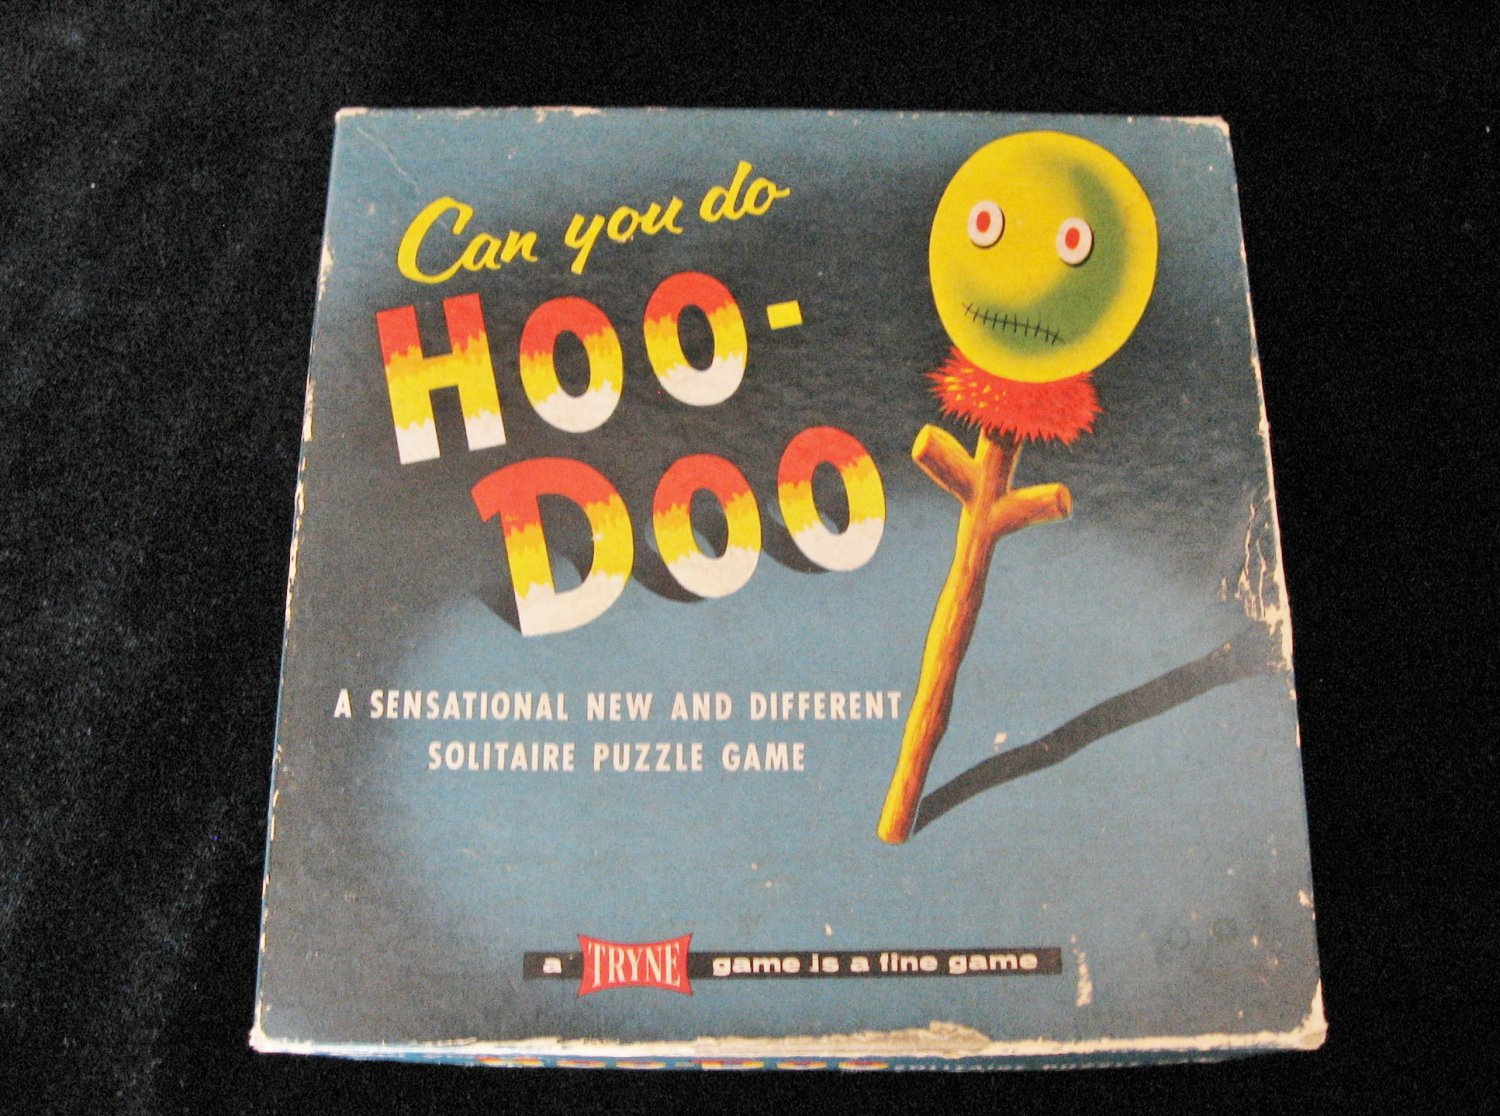
\includegraphics[width=5cm]{hoodoo2.jpg}
    \label{fig:capa original}
}
\quad\quad\quad
\subfloat[Regras]{
    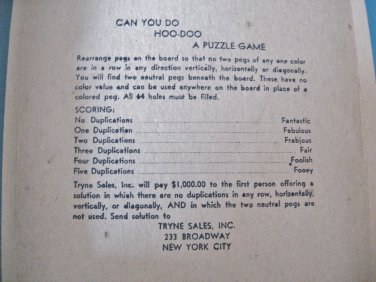
\includegraphics[width=5cm]{regras.jpg}
    \label{fig:regras}
}
\end{figure}
\newpage
\section{Vari\'{a}veis de Decis\~{a}o}

Para modelar o problema em causa, usamos uma vari\'{a}vel por cada posi\c{c}\~{a}o no tabuleiro, perfazendo para um tabuleiro $n * m$ (onde n \'{e} a altura do tabuleiro e m \'{e} a largura do mesmo), $n * m$ vari\'{a}veis.O dom\'{i}nio dessas vari\'{a}veis depende tamb\'{e}m ele do tamanho do tabuleiro, sendo que existem para cada tipo de tabuleiro dois dom\'{i}nios distintos dependendo de o jogo ser resolvido usando pe\c{c}as transparentes ou n\~{a}o.
Para o caso de serem usadas pe\c{c}as transparentes o dom\'{i}nio de cada uma das vari\'{a}veis \'{e} $[0,n]$ (assumindo que n \'{e} a maior dimens\~{a}o do tabuleiro).
No caso de se recorrer somente a pe\c{c}as com cor o dom\'{i}nio de cada uma das vari\'{a}veis passa a ser $[1,n]$ (assumindo que n \'{e} a maior dimens\~{a}o do tabuleiro).

No caso de o jogo ser resolvido recorrendo aos \emph{pegs} transparentes \'{e} ainda utilizada uma vari\'{a}vel extra, vari\'{a}vel essa que conta o n\'{u}mero de \emph{pegs} transparentes no tabuleiro. O dom\'{i}mio desta vari\'{a}vel vai desde zero at\'{e} $n*m$, caso em que todas as pe\c{c}as do tabuleiro s\~{a}o \emph{pegs} transparentes.

\section{Restri\c{c}\~{o}es}

Tratando-se de um jogo todas as restri\c{c}\~{o}es que inclu\'{i}mos s\~{a}o r\'{i}gidas, \`{a} excep\c{c}\~{a}o de uma.
As restri\c{c}\~{o}es r\'{i}gidas s\~{a}o:

\begin{itemize}
\item A restri\c{c}\~{a}o que impede que duas pe\c{c}as da mesma linha tenham valores iguais;
\item A restri\c{c}\~{a}o que impede que duas pe\c{c}as da mesma coluna tenham valores iguais;
\item A restri\c{c}\~{a}o que impede que duas pe\c{c}as da mesma diagonal tenham valores iguais;
\end{itemize}

A restri\c{c}\~{a}o flex\'{i}vel, diz respeito \'{a} tentativa de minimizar o n\'{u}mero de pe\c{c}as transparentes envolvidas na resolu\c{c}\~{a}o do tabuleiro (que \'{e} por si tamb\'{e}m um dos objectivos do jogo).

A implementa\c{c}\~{a}o das restri\c{c}\~{o}es r\'{i}gidas \'{e} feita agrupando as vari\'{a}veis em listas, ora por linha, ora por coluna, ora por diagonal , e chamando o predicado \emph{all\_distinct} sobre essas listas, obrigando assim que nunca haja duas pe\c{c}as que partilhem a mesma linha/coluna/diagonal que tenham o mesmo valor.

A implementa\c{c}\~{a}o da restri\c{c}\~{a}o flex\'{i}vel, \'{e} feita pela introdu\c{c}\~{a}o de uma vari\'{a}vel antes do \emph{labeling}, a qual se passa ao predicado \emph{count} , com o intuito de contar o n\'{u}mero de pe\c{c}as com valor zero no tabuleiro (n\'{u}mero de pegs transparentes).

Esta \'{u}ltima restri\c{c}\~{a}o, \'{e} implementada por meio da tentativa de minimiza\c{c}\~{a}o do valor da vari\'{a}vel supra mencionada. Este efeito \'{e} conseguido passando como op\c{c}\~{a}o de \emph{labeling} o predicado \emph{minimize} passando-lhe a vari\'{a}vel criada propositadamente para o efeito. Esta restri\c{c}\~{a}o permite assim tentar sempre obter a solu\c{c}\~{a}o para o tabuleiro que usa menos \emph{pegs} transparentes.  

\section{Estrat\'{e}gia de Pesquisa}


Na estrat\'{e}gia de pesquisa utilizada, quanto o jogo \'{e} jogado com a possibilidade de introduzir \emph{pegs} transparentes, optamos por incluir as seguintes op\c{c}\~{o}es para a etiquetarem das vari\'{a}veis:

\begin{itemize}
\item \emph{down} : permitindo assim que o dom\'{i}nio seja percorrido em ordem descendente;
\item \emph{minimize(X)} : para aplicar a restri\c{c}\~{a}o flex\'{i}vel ;
\item \emph{time\_out(Time,Flags)} : para evitar que a execu\c{c}\~{a}o se prolongue por tempo indeterminado;
\item \emph{ffc} : para tentar falhar o mais rapidamente poss\'{i}vel,"cortando" a \`{a}rvore de pesquisa mais cedo e eliminando assim mais n\'{os};
\end{itemize}

O \emph{down} foi utilizado por raz\~{o}es obvias: como as \emph{pegs} transparentes s\~{a}o codificadas com o n\'{u}mero zero, e como o dom\'{i}nio das vari\'{a}veis vai tipicamente de zero at\'{e} n, em que n \'{e} o lado do tabuleiro, ao percorrer o dom\'{i}nio de valores maiores at\'{e} zero obtemos melhores resultados mais r\'{a}pidamente em geral. Isto tendo em conta que uma melhor solu\c{c}\~{a}o \'{e} aquela que usa menos \emph{pegs} transparentes.

O \emph{minimize(X)} foi tamb\'{e}m ele utilizado por raz\~{o}es j\'{a} explicadas anteriormente, que se prendem com a necessidade de tentar encontrar a solu\c{c}\~{a}o que minimiza o n\'{u}mero de \emph{pegs} transparentes. Nesse sentido a vari\'{a}vel que \'{e} passada ao predicado \emph{minimize(X)} \'{e} a vari\'{a}vel que conta o n\'{u}mero de zeros no tabuleiro. 

O predicado \emph{time\_out(Time,Flags)} \'{e} usado para que a execu\c{c}\~{a}o n\~{a}o decorra indeterminadamente. Com esse fim \'{e} passado ao predicado o valor de \emph{120000} que faz com que o \emph{labeling} decorra  durante no m\'{a}ximo 2 minutos e retorne ent\~{a}o, sen\~{a}o antes, a melhor solu\c{c}\~{a}o at\'{e} ao momento.

A op\c{c}\~{a}o \emph{ffc} foi utilizada na tentativa de tentar que fossem atribu\'{i}dos primeiro valores as vari\'{a}veis mais restritas, tentando assim "cortar" mais ramos da \'{a}rvore de pesquisa, ao falhar mais cedo.

Como \'{e} referido na sec\c{c}\~{a}o pr\'{o}pria, verificamos que a utiliza\c{c}\~{a}o de outras op\c{c}\~{o}es como por exemplo \emph{bisect} , resulta em resultados ligeiramente menos satisfat\'{o}rios.

Quando \'{e} usado o \emph{bisect} a performance \'{e} sensivelmente pior do que no caso de se usar a sele\c{c}\~{a}o de valores por defeito, provavelmente porque o beneficio que tr\'{a}s \'{e} quase nulo, e o custo do seu calculo \'{e} naturalmente algum, ainda que diminuto, causando ent\~{a}o uma pequena degrada\c{c}\~{a}o da performance.


\section{Visualiza\c{c}\~{a}o}

Existem seis predicados utilizados para a constru\c{c}\~{a}o visual do tabuleiro em modo de texto. O primeiro predicado a ser executado \'{e} o \textit{print\_tab(+board)} que recebe como argumento um tabuleiro representado por uma lista de listas de inteiros. Este predicado calcula o comprimento da lista, e das sub-listas. Obtidos os n\'{u}meros de linhas e colunas do tabuleiro em quest\~{a}o, procede-se \`{a} impress\~{a}o. Enquanto a cauda da lista n\~{a}o for vazia, isto \'{e}, ainda existirem mais linhas, segue-se um procedimento b\'{a}sico, que consiste em imprimir primeiro uma linha horizontal, numa nova linha verificar o tamanho do \'{i}ndice, para calcular o n\'{u}mero de caracteres vazios a escrever entre o \'{i}ndice e in\'{i}cio do tabuleiro(este processo de escalonamento do espa\c{c}o para alinha a impress\~{a}o tamb\'{e}m \'{e} usado para os valores das pegs no interior do tabuleiro), e s\'{o} de seguida \'{e} impressa a linha de valores, que \'{e} a primeira lista. Este ciclo repete-se at\'{e} chegar ent\~{a}o \`{a} situa\c{c}\~{a}o onde a cauda da lista \'{e} vazia. 
\paragraph*{}
Quando a cauda da lista \'{e} vazia, a primeira parte do processo mant\'{e}m-se(impress\~{a}o da linha horizontal, e tamb\'{e}m dos valores com o respectivo alinhamento), mas ap\'{o}s a impress\~{a}o dos valores da lista, \'{e} de imediato impressa outra linha horizontal e seguida do \'{i}ndice das colunas com valores Alfa-num\'{e}ricos. 
Vemos em baixo um exemplo de tabuleiro impresso na consola:
\paragraph*{}


\begin{figure}[h!]
\begin{center}
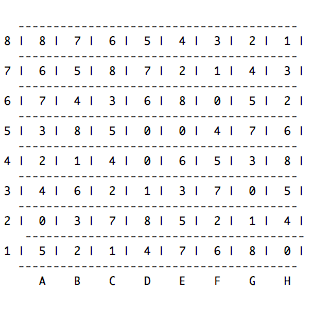
\includegraphics[scale=0.5]{tabuleiro.png}
\caption{\textit{Tabuleiro 8x8 resolvido}}
\label{fig:jogo_original}
\end{center}
\end{figure}







\section{Resultados}

No processo de desenvolvimento do solver fizemos v\'{a}rios testes utilizando v\'{a}rias op\c{c}\~{o}es de etiquetarem das vari\'{a}veis, por forma a tentar obter o melhor resultado poss\'{i}vel, o mais rapidamente poss\'{i}vel, na maioria dos casos.
O estudo que fizemos, centrou-se principalmente no caso em que \'{e} poss\'{i}vel usar \emph{pegs} transparentes, tentando no entanto minimizar o seu uso, por este ser o caso mais interessante.
Dividimos o estudo em duas partes, na primeira parte analisamos o comportamento das v\'{a}rias op\c{c}\~{o}es tendo em conta par\^{a}metros como o n\'{u}mero de \emph{backtracks} ou o tempo de execu\c{c}\~{a}o, sendo este estudo feito para aqueles tabuleiros com que conseguimos garantidamente alcan\c{c}ar uma solu\c{c}\~{a}o optima.
A segunda parte do estudo consistiu na compara\c{c}\~{a}o do n\'{u}mero de \emph{pegs} transparentes utilizado na resolu\c{c}\~{a}o de alguns dos problemas para os quais n\~{a}o temos uma solu\c{c}\~{a}o optima, isto utilizando tamb\'{e}m diferentes op\c{c}\~{o}es de etiquetagem.
Esta divis\~{a}o deveu-se a que, em problemas em que a solu\c{c}\~{a}o encontrada n\~{a}o \'{e} optima, de pouco interessa saber m\'{e}tricas como o n\'{u}mero de \emph{backtracks} ou o tempo de execu\c{c}\~{a}o (que ser\'{a} sempre o mesmo), interessa ao inv\'{e}s disso saber qual a melhor solu\c{c}\~{a}o de todas as encontradas com as diversas op\c{c}\~{o}es.

No que diz respeito aos problemas para os quais se tem uma resolu\c{c}\~{a}o optima, verificou-se que o \emph{down} leva \`{a} mais r\'{a}pida resolu\c{c}\~{a}o do problema na maior parte dos casos. Facto que pode ser verificado comparando os dados das tabelas \ref{tabela:1}, \ref{tabela:2}, \ref{tabela:3} e \ref{tabela:4} (em anexo). Isto no entanto n\~{a}o se verifica para tamanhos de tabuleiros maiores, nomeadamente, para tamanhos superiores a 6x6, onde a etiquetagem com as op\c{c}\~{o}es \emph{down} e \emph{ffc} revela-se a mais r\'{a}pida e a que tem consistentemente melhores resultados. Esse facto come\c{c}a-se a observar no tabuleiro 7x7 onde a etiquetagem com as op\c{c}\~{o}es supra referidas come\c{c}a j\'{a} a ser melhor e mais r\'{a}pida que as outras, resultando em que o tempo de execu\c{c}\~{a}o seja menor, isto embora o n\'{u}mero de \emph{prunings} seja menor e o n\'{u}mero de \emph{backtracks} maior. Esta tend\^{e}ncia torna-se evidente para os tabuleiros de maior tamanho onde nunca se chega a alcan\c{c}ar uma solu\c{c}\~{a}o optima mas, onde os resultados da etiquetarem com as op\c{c}\~{o}es \emph{down} e \emph{ffc} d\~{a}o solu\c{c}\~{o}es francamente melhores. Esses factos podem ser observados principalmente nas tabelas \ref{tabela:5}, \ref{tabela:6}, \ref{tabela:7}, \ref{tabela:8} e \ref{tabela:9}, tabelas essas onde se mostram o n\'{u}mero de \emph{pegs} transparentes utilizadas em resolu\c{c}\~{o}es com alguns tempos de dura\c{c}\~{a}o m\'{a}ximos selecionados. Nessas tabelas \'{e} not\'{o}rio o beneficio de usar a combina\c{c}\~{a}o de op\c{c}\~{o}es supra mencionadas pois produzem consistentemente resolu\c{c}\~{o}es melhores (com menos \emph{pegs} transparentes) e mais cedo do que as outras combina\c{c}\~{o}es. Esse facto \'{e} tamb\'{e}m aludido nos gr\'{a}ficos apresentados, (\ref{graf1}, \ref{graf2} e \ref{graf3} ), onde se pode ver que claramente a pior op\c{c}\~{a}o de entre as testadas \'{e} utilizar os par\^{a}metros por defeito, que retornam consistentemente piores resultados que qualquer uma das outras op\c{c}\~{o}es. De entre as outras op\c{c}\~{o}es na grande maioria dos casos, a alternativa que usa as op\c{c}\~{o}es \emph{down} juntamente com \emph{ffc} obtem ligeiramente melhores resultados.
A op\c{c}\~{a}o de usar a combina\c{c}\~{a}o de op\c{c}\~{o}es \emph{down} com \emph{ffc} e \emph{bisect} em simult\^{a}neo (n\~{a}o inclu\'{i}da em nenhum dos gr\'{a}ficos por uma quest\~{a}o de clareza dos mesmo) foi estudada com a ajuda da tabela \ref{tabela:9}, no entanto os resultados que se conseguem obter s\~{a}o em tudo semelhantes aos em que se obtem quando se utiliza somente \emph{down} e \emph{ffc}, sendo que em alguns casos tem resultados ligeiramente piores, e noutros ligeiramente melhores, pelo que n\~{a}o \'{e} uma op\c{c}\~{a}o claramente vantajosa.

Apesar da tentativa de contacto com colegas de outros grupos, com vista \'{a} troca de resultados, obtivemos apenas uma resposta, de um colega que utilizou uma abordagem muito diferente da nossa que n\~{a}o permite portanto fazer uma compara\c{c}\~{a}o dos resultados.

\section{Conclus\~{o}es}

Com a realiza\c{c}\~{a}o do presente trabalho pud\'{e}mos verificar a simplicidade e eleg\^{a}ncia com que, a programa\c{c}\~{a}o em l\'{o}gica com restri\c{c}\~{o}es, nos permite implementar solu\c{c}\~{o}es para problemas como o \emph{Hoo$-$Doo}.
A implementa\c{c}\~{a}o \'{e} n\~{a}o s\'{o} compacta, facilmente leg\'{i}vel, como \'{e} tamb\'{e}m de uma eleg\^{a}ncia e simplicidade que n\~{a}o seria facilmente alcan\c{c}avel com o uso de uma linguagem imperativa como \emph{C} ou \emph{Java}.
Parece-nos no entanto, que essa simplicidade acarreta alguns custos a n\'{i}vel de performance, uma vez que nos parece, isto no entanto sem termos dados concretos que sustentem esta hip\'{o}tese, que uma implementa\c{c}\~{a}o numa linguagem imperativa do tipo \emph{C}, utilizando um algoritmo adequado, teria uma performance bastante melhor.
\'{E} no entanto indiscut\'{i}vel, a vantagem de utilizar PLR nesta situa\c{c}\~{a}o, uma vez que a implementa\c{c}\~{a}o do \emph{solver} \'{e} muito mais simples e clara.
Tivemos ainda oportunidade de atestar a versatilidade que as op\c{c}\~{o}es do predicado \emph{labeling} trazem \'{a} resolu\c{c}\~{a}o deste tipo de problemas, dotando o programador da possibilidade de fazer pequenos ajustes que permitem melhorar dramaticamente a performance do programa.
Caso tiv\'{e}ssemos tido mais tempo poder\'{i}amos eventualmente fazer uma r\'{a}pida implementa\c{c}\~{a}o de um solver numa linguagem imperativa, para termos uma no\c{c}\~{a}o mais exacta de quais as diferen\c{c}as em termos de performance que existem entre estes dois tipos de abordagens, atestando assim a aplicabilidade e utilidade da PLR em situa\c{c}\~{o}es semelhantes a esta.
\nocite{sicstusManual}
\nocite{hooDoo}



\clearpage
\addcontentsline{toc}{section}{Bibliografia}
\renewcommand\refname{Bibliografia}
\bibliographystyle{plain}
\bibliography{refs.bib}


\newpage
\appendix


\section{Codigo}
\subsection{Hoo\-Doo.pro}
\lstinputlisting{HooDoo.pro}

\subsection{custom\_all\_distinct.pro}
\lstinputlisting{custom_all_distinct.pro}

\subsection{flat\_2D\_convert.pro}
\lstinputlisting{flat_2D_convert.pro}

\subsection{tabPrint.pro}
\lstinputlisting{tabPrint.pro}

\newpage
\section{Tabelas e Gr\'{a}ficos}

\setlength{\tabcolsep}{12pt}
\begin{table}[ht] 
\caption{Problemas com solu\c{c}\~{a}o optima : Op\c{c}\~{o}es por defeito} % title of Table 
\centering % used for centering table 
\begin{tabular}{c c c c c c} % centered columns (4 columns) 
\hline\hline %inserts double horizontal lines 

M\'{e}trica & 2x2 & 3x3 & 4x4 & 5x5 & 7x7\\ [0.5ex] % inserts table 
%heading 
\hline % inserts single horizontal line 
Runtime & 10 & 10 & 125 & 10 & 10900 \\ % inserting body of the table 
Resumptions & 304 & 9141 & 478328 & 16882 & 33054848 \\ 
Entailments & 161 & 4669 & 234053 & 9878 & 29865115  \\ 
Prunings & 205 & 5126 & 240508 & 10307 & 17858406 \\ 
Backtracks & 8 & 129 & 3194 & 194 & 346785 \\ 
Constraints & 27 & 103 & 261 & 531 & 1527 \\ [1ex] % [1ex] adds vertical space 
\hline %inserts single line 
\end{tabular} 
\label{tabela:1} % is used to refer this table in the text 
\end{table}


\setlength{\tabcolsep}{12pt}
\begin{table}[ht] 
\caption{Problemas com solu\c{c}\~{a}o optima : Op\c{c}\~{a}o \emph{down}} % title of Table 
\centering % used for centering table 
\begin{tabular}{c c c c c c} % centered columns (4 columns) 
\hline\hline %inserts double horizontal lines 

M\'{e}trica & 2x2 & 3x3 & 4x4 & 5x5 & 7x7\\ [0.5ex] % inserts table 
%heading 
\hline % inserts single horizontal line 
Runtime & 10 & 10 & 125 & 10 & 10900 \\
Resumptions & 304 & 9141 & 478328 & 16882 & 33054848 \\
Entailments & 161 & 4669 & 234053 & 9878 & 29865115 \\
Prunings & 205 & 5126 & 240508 & 10307 & 17858406 \\
Backtracks & 8 & 129 & 3194 & 194 & 346785 \\
Constraints & 27 & 103 & 261 & 531 & 1527 \\[1 ex]
\hline %inserts single line 
\end{tabular} 
\label{tabela:2} % is used to refer this table in the text 
\end{table}

\setlength{\tabcolsep}{12pt}
\begin{table}[ht] 
\caption{Problemas com solu\c{c}\~{a}o optima : Op\c{c}\~{o}es \emph{down} e \emph{ffc}} % title of Table 
\centering % used for centering table 
\begin{tabular}{c c c c c c} % centered columns (4 columns) 
\hline\hline %inserts double horizontal lines 

M\'{e}trica & 2x2 & 3x3 & 4x4 & 5x5 & 7x7\\ [0.5ex] % inserts table 
%heading 
\hline % inserts single horizontal line 
Runtime & 10 & 10 & 90 & 10 & 59180 \\
Resumptions & 286 & 7667 & 268519 & 14254 & 295555138 \\
Entailments & 134 & 3776 & 139331 & 6073 & 127518166 \\
Prunings & 177 & 4180 & 139466 & 6244 & 118181814 \\
Backtracks & 5 & 90 & 1748 & 107 & 1727869 \\
Constraints & 27 & 103 & 261 & 531 & 1527 \\[1 ex]
\hline %inserts single line 
\end{tabular} 
\label{tabela:3} % is used to refer this table in the text 
\end{table}

\setlength{\tabcolsep}{12pt}
\begin{table}[ht] 
\caption{Problemas com solu\c{c}\~{a}o optima : Op\c{c}\~{o}es \emph{down} e \emph{bisect}} % title of Table 
\centering % used for centering table 
\begin{tabular}{c c c c c c} % centered columns (4 columns) 
\hline\hline %inserts double horizontal lines 

M\'{e}trica & 2x2 & 3x3 & 4x4 & 5x5 & 7x7\\ [0.5ex] % inserts table 
%heading 
\hline % inserts single horizontal line 
Runtime & 10 & 10 & 80 & 10 & 117930 \\
Resumptions & 286 & 8438 & 277571 & 9634 & 491394424 \\
Entailments & 134 & 4114 & 133215 & 3656 & 249165687 \\
Prunings & 182 & 4565 & 136734 & 3896 & 225597907 \\
Backtracks & 5 & 102 & 1611 & 51 & 1036895 \\
Constraints & 27 & 103 & 261 & 531 & 1527 \\[1 ex]
\hline %inserts single line 
\end{tabular} 
\label{tabela:4} % is used to refer this table in the text 
\end{table}





\setlength{\tabcolsep}{12pt}
\begin{table}[ht] 
\caption{N\'{u}mero de \emph{pegs} transparentes usadas apos timeout : Op\c{c}\~{o}es por defeito} % title of Table 
\centering % used for centering table 
\begin{tabular}{c c c c c c c} % centered columns (4 columns) 
\hline\hline %inserts double horizontal lines 

Tempo(s) & 6x6 & 8x8 & 9x9 & 10x10 & 11x11 & 20x20\\ [0.5ex] % inserts table 
%heading 
\hline % inserts single horizontal line 
2 & 7 & 11 & 18 & 25 & 32 & 265 \\
10 & 7 & 8 & 16 & 22 & 30 & 248 \\
120 & 6 & 8 & 13 & 21 & 24 & 185 \\[1 ex]
\hline %inserts single line 
\end{tabular} 
\label{tabela:5} % is used to refer this table in the text 
\end{table}


\setlength{\tabcolsep}{12pt}
\begin{table}[ht] 
\caption{N\'{u}mero de \emph{pegs} transparentes usadas apos timeout : Op\c{c}\~{o}es \emph{down}} % title of Table 
\centering % used for centering table 
\begin{tabular}{c c c c c c c} % centered columns (4 columns) 
\hline\hline %inserts double horizontal lines 

Tempo(s) & 6x6 & 8x8 & 9x9 & 10x10 & 11x11 & 20x20\\ [0.5ex] % inserts table 
%heading 
\hline % inserts single horizontal line 
2 & 6 & 11 & 16 & 21 & 26 & 79 \\
10 & 4 & 11 & 16 & 20 & 26 & 78 \\
120 & 4 & 7 & 15 & 19 & 26 & 78 \\[1 ex]
\hline %inserts single line 
\end{tabular} 
\label{tabela:6} % is used to refer this table in the text 
\end{table}


\setlength{\tabcolsep}{12pt}
\begin{table}[ht] 
\caption{N\'{u}mero de \emph{pegs} transparentes usadas apos timeout : Op\c{c}\~{o}es \emph{down} e \emph{ffc}} % title of Table 
\centering % used for centering table 
\begin{tabular}{c c c c c c c} % centered columns (4 columns) 
\hline\hline %inserts double horizontal lines 

Tempo(s) & 6x6 & 8x8 & 9x9 & 10x10 & 11x11 & 20x20\\ [0.5ex] % inserts table 
%heading 
\hline % inserts single horizontal line 
2 & 5 & 11 & 12 & 17 & 21 & 68 \\
10 & 4 & 11 & 11 & 17 & 21 & 68 \\
120 & 4 & 11 & 11 & 16 & 21 & 67 \\[1 ex]
\hline %inserts single line 
\end{tabular} 
\label{tabela:7} % is used to refer this table in the text 
\end{table}


\setlength{\tabcolsep}{12pt}
\begin{table}[ht!] 
\caption{N\'{u}mero de \emph{pegs} transparentes usadas apos timeout : Op\c{c}\~{o}es \emph{down} e \emph{bisect}} % title of Table 
\centering % used for centering table 
\begin{tabular}{c c c c c c c} % centered columns (4 columns) 
\hline\hline %inserts double horizontal lines 

Tempo(s) & 6x6 & 8x8 & 9x9 & 10x10 & 11x11 & 20x20\\ [0.5ex] % inserts table 
%heading 
\hline % inserts single horizontal line 
2 & 6 & 11 & 16 & 21 & 26 & 78 \\
10 & 4 & 11 & 16 & 20 & 26 & 78 \\
120 & 4 & 7 & 15 & 19 & 24 & 78 \\[1 ex]
\hline %inserts single line 
\end{tabular} 
\label{tabela:8} % is used to refer this table in the text 
\end{table}


\setlength{\tabcolsep}{12pt}
\begin{table}[ht!] 
\caption{N\'{u}mero de \emph{pegs} transparentes usadas apos timeout : Op\c{c}\~{o}es \emph{down}, \emph{bisect} e \emph{ffc}} % title of Table 
\centering % used for centering table 
\begin{tabular}{c c c c c c c} % centered columns (4 columns) 
\hline\hline %inserts double horizontal lines 

Tempo(s) & 6x6 & 8x8 & 9x9 & 10x10 & 11x11 & 20x20\\ [0.5ex] % inserts table 
%heading 
\hline % inserts single horizontal line 
2 & 5 & 11 & 12 & 18 & 21 & 68 \\
10 & 4 & 11 & 11 & 18 & 21 & 67 \\
120 & 4 & 11 & 11 & 17 & 21 & 67 \\[1 ex]
\hline %inserts single line 
\end{tabular} 
\label{tabela:9} % is used to refer this table in the text 
\end{table}



\begin{figure}[ht]
\centering
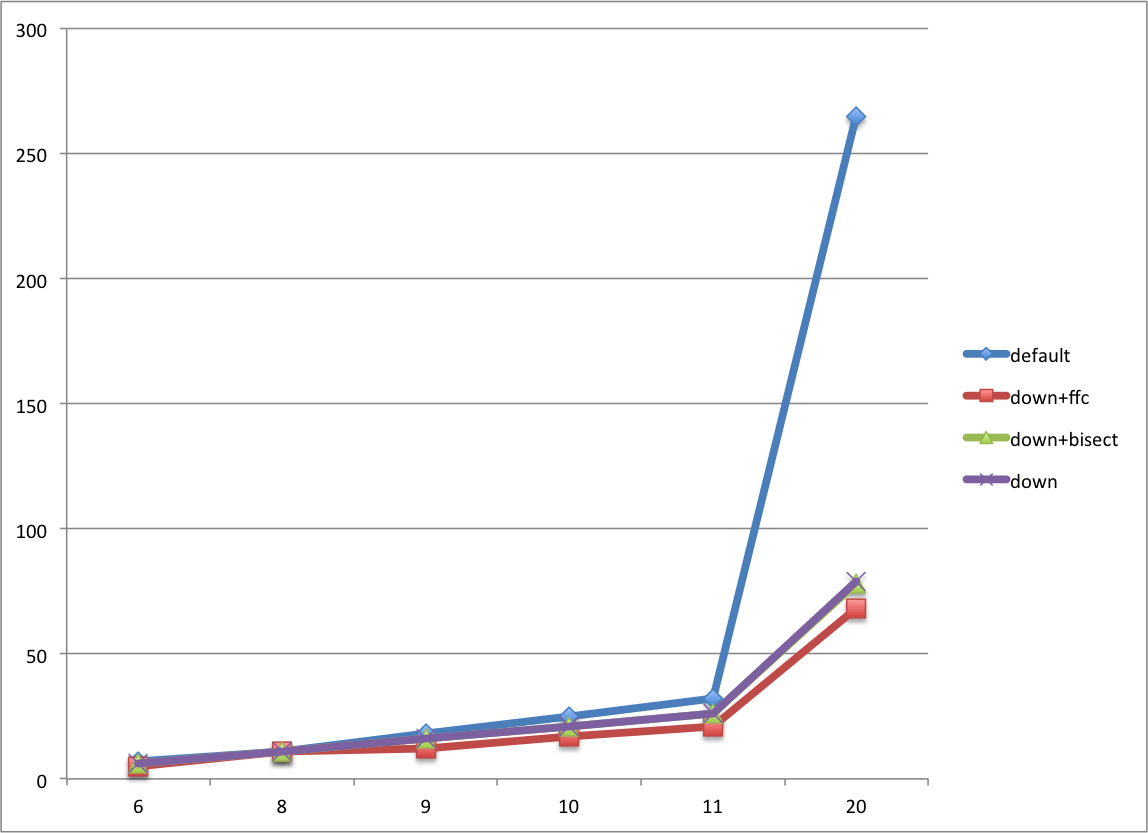
\includegraphics[width=90mm]{grafico3.png}
\caption{N\'{u}mero de \emph{pegs} transparentes ao fim de 1 segundo}
\label{graf1}
\end{figure}


\begin{figure}[ht]
\centering
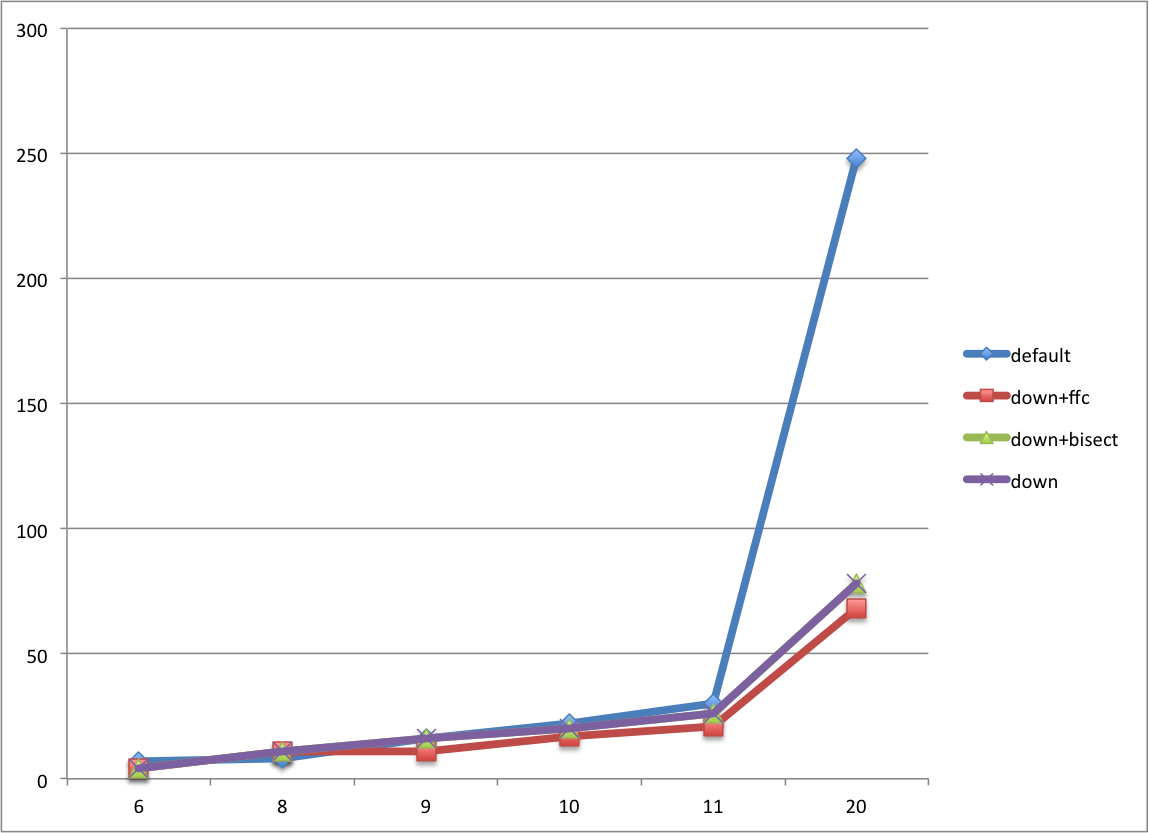
\includegraphics[width=90mm]{grafico2.png}
\caption{N\'{u}mero de \emph{pegs} transparentes ao fim de 2 segundos}
\label{graf2}
\end{figure}


\begin{figure}[ht]
\centering
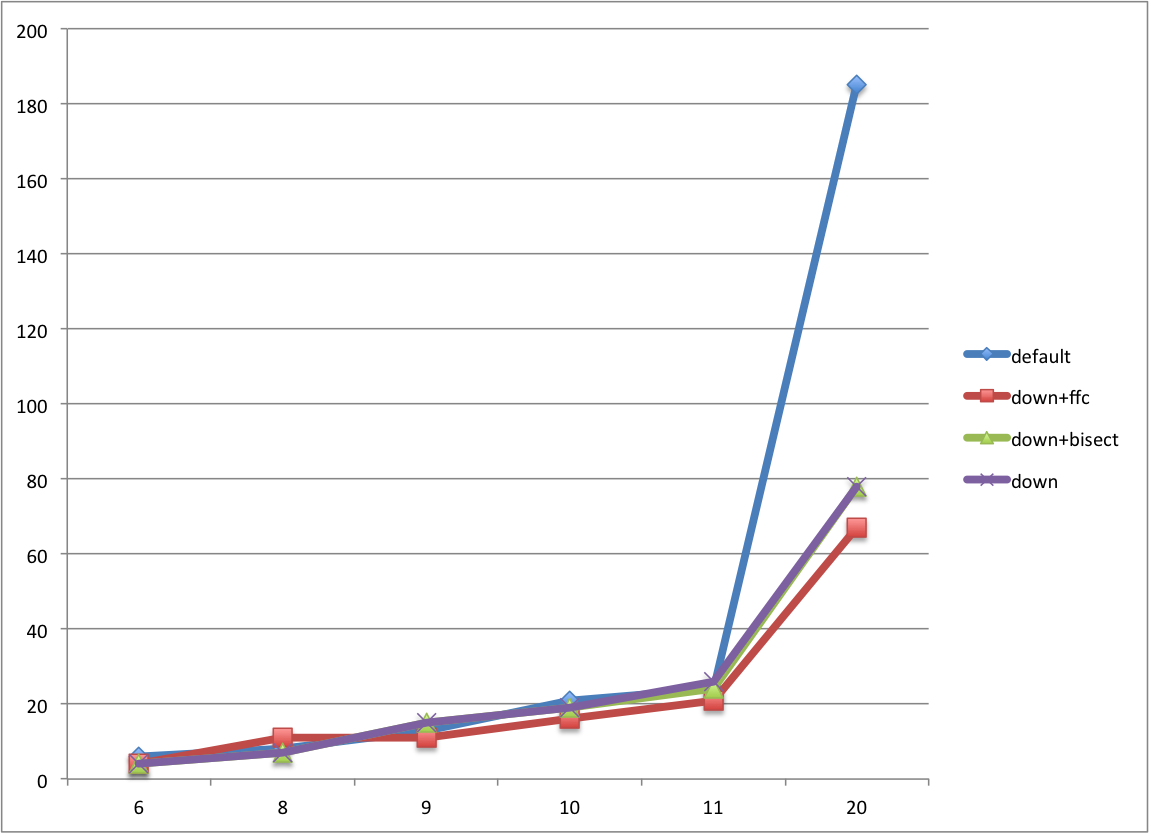
\includegraphics[width=90mm]{grafico1.png}
\caption{N\'{u}mero de \emph{pegs} transparentes ao fim de 2 minutos}
\label{graf3}
\end{figure}









\end{document}